\subsubsection*{Partie A}
Un club de vacances propose deux types d'activités à ses clients : des randonnées le matin et des activités nautiques l'après-midi.

\vspace{5mm}
On sait que
\begin{itemize}[label=$\bullet$]
	\item un quart des clients participent aux randonnées.
	\item parmi les clients ayant choisi de faire une randonnée le matin, la moitié s'inscrit aussi aux activités nautiques de l'après-midi.
	\item parmi les clients n'ayant pas choisi de faire une randonnée le matin, un tiers s'inscrit aux activités nautiques de l'après-midi.
\end{itemize}

On choisit un client du club de vacances au hasard et on note :
\begin{itemize}[label=$\bullet$]
\item \textit{R} l'événement: \og{}le client participe à la randonnée\fg{}.

\item \textit{N} l'événement : \og{}le client participe aux activités nautiques\fg{}.
\end{itemize}
\begin{enumerate}
	\item Recopier et compléter l'arbre de probabilité représentant la situation.


\begin{minipage}[t]{0.45\linewidth}\vspace{0mm}
			\textcolor{red}{\textsc{Correction}}\\
	Un quart des clients participent aux randonnées, donc \mbox{$P (R)=\dfrac14$} et \mbox{$P (\overline{R})=\dfrac34$}.

	La moitié de ceux qui ont fait une randonnée font des activités nautiques, donc \mbox{$P_R (N)=\dfrac12$} et \mbox{$P_R (\overline{N})=\dfrac12$}.

	Un tiers de ceux qui n'ont pas randonné font des activités nautiques, donc \mbox{$P_{\overline{R}} (N)=\dfrac13$} et \mbox{$P_{\overline{R}} (\overline{N})=\dfrac23$}.

\end{minipage}\hspace{0.05\linewidth}\begin{minipage}[t]{0.45\linewidth}\vspace{0mm}


			\begin{tikzpicture}[xscale=1,yscale=1,rotate=0,every node/.style={scale=1,rotate=0}]
			\node(n0)at(0,0){};
			\node(n1_1)at(3,1){$R$};
			\node(n1_2)at(3,-1){$\overline{R}$};
			\node(n2_1)at(6,1.5){$N$};
			\node(n2_2)at(6,0.5){$\overline{N}$};
			\node(n2_3)at(6,-0.5){$N$};
			\node(n2_4)at(6,-1.5){$\overline{N}$};
			\draw[blue](n0)--(n1_1)node[pos=0.6,fill=white]{$\dfrac14$};
			\draw[blue](n0)--(n1_2)node[pos=0.4,fill=white]{$\dfrac34$};
			\draw[blue](n2_1)--(n1_1)node[pos=0.6,fill=white]{$\dfrac12$};
			\draw[blue](n2_2)--(n1_1)node[pos=0.4,fill=white]{$\dfrac12$};
			\draw[blue](n2_3)--(n1_2)node[pos=0.6,fill=white]{$\dfrac13$};
			\draw[blue](n2_4)--(n1_2)node[pos=0.4,fill=white]{$\dfrac23$};

		\end{tikzpicture}
\end{minipage}


		\item Montrer que la probabilité que le client participe aux activités nautiques est de \mbox{$\dfrac38$}.

				\textcolor{red}{\textsc{Correction}}\\
				Loi des probabilités totales : \mbox{$P(N)=P(R\cap N)+P(\overline{R}\cap N)$}.

				Donc \mbox{$P(N)=\dfrac14\times\dfrac12+\dfrac34\times\dfrac13=\dfrac18+\dfrac14=\dfrac38$}.

				La  probabilité que le client participe aux activités nautiques est de \mbox{$\dfrac38$}.

\item Sachant que le client a participé aux activités nautiques de l'après-midi, quelle est la probabilité qu'il ait fait la randonnée du matin ?

				\textcolor{red}{\textsc{Correction}}\\

				On cherche \mbox{$P_N (R)$}.

				Règle des probabilités conditionnelles : \mbox{$P_N (R)=\dfrac{P(R \cap N)}{P(N)}=\dfrac{\frac18}{\frac38}=\dfrac18\times\dfrac83=\dfrac13$}.

				La probabilité qu'un client, choisi parmi ceux qui font des activités nautiques, ait fait une randonnée le matin est $\dfrac13$.
		\item Les événements \textit{R} et \textit{N} sont-ils indépendants ? Justifier.

						\textcolor{red}{\textsc{Correction}}\\
						Pas du tout, puisque \mbox{$P(R \cap N)=\dfrac18$}, alors que \mbox{$P(R)\times P(N)=\dfrac14\times\dfrac38=\dfrac{3}{32}$}.
	\end{enumerate}
\subsubsection*{Partie B}
En 2025, le club a accueilli 400 clients. Son directeur projette la fréquentation du club dans les années à venir en modélisant le nombre de clients du club les années suivantes par la suite \mbox{$(u_n)$} définie par :

\begin{center}
	\mbox{$u_0=400$} et pour tout entier naturel $n$, \mbox{$u_{n+1}=\np{1.025}u_n$}
\end{center}

où $u_n$ représente le nombre de clients du club pour l'année \mbox{$2025+n$}
\begin{enumerate}
	\item Donner la nature de la suite $(u_n)$ en précisant sa raison.

					\textcolor{red}{\textsc{Correction}}\\
					$(u_n)$ est une suite géométrique de raison \np{1.025}.
	\item Selon ce modèle; quel est le taux d'évolution annuel de la fréquentation de ce club de vacances ?

					\textcolor{red}{\textsc{Correction}}\\
					La multiplication par \np{1.025} correspond à une augmentation, exprimée en pourcentage, de \np{2.5}\% : le taux d'évolution annuel de la fréquentation est \np{2.5}\%.
	\item
	 \begin{enumerate}
	\item
	\begin{minipage}[t]{0.66\linewidth}\vspace{0mm}
		Recopier et compléter la fonction \texttt{seuil}, codée en python, afin qu'elle renvoie la plus petite valeur de $n$ telle que $u_n$ soit supérieure ou égale à $k$, où $k$ est un entier naturel non nul.

				\textcolor{red}{\textsc{Correction}}\\
				La boucle \og{}tourne\fg{} aussi longtemps que $u$ est inférieur à $k$.

				A chaque itération, on incrémente $n$, et on calcule la nouvelle valeur de $u$ en utilisant \underline{la relation de récurrence}.
\end{minipage}
\hspace{0.05\linewidth}
	\begin{minipage}[t]{0.33\linewidth}\vspace{0cm}
	\begin{ttfamily}
\begin{tblr}{hline{1,Z}={solid}, vlines,colspec={X},rowsep=0pt}
	def seuil (k) :\\
	\qquad u = 400\\
	\qquad n = 0\\
	\qquad while  \textcolor{red}{u < k} :\\
	\qquad\qquad  n = \textcolor{red}{n+1}\\
	\qquad\qquad  u= \textcolor{red}{u * 1.025}\\
	\qquad return \textcolor{red}{n}\\
\end{tblr}
\end{ttfamily}
\end{minipage}


	\item
\begin{minipage}[t]{0.45\linewidth}\vspace{0mm}
Le tableau ci-contre a été extrait d'une feuille automatisée de calcul donnant les valeurs arrondies au centième de \mbox{$\np{1.025}^n$} pour certaines valeurs de $n$.

	\vspace{5mm}
	Déterminer la valeur renvoyée par \texttt{seuil(600)}, où \texttt{seuil} est la fonction codée en python donnée en 3.a).


		\vspace{5mm}
	Interpréter ce résultat dans le contexte de l'exercice.


		\vspace{5mm}
				\textcolor{red}{\textsc{Correction}}\\

				Pour que l'on atteigne 600 clients, il faut que \mbox{$\np{1.025}^n$} dépasse \np{1.5}.

				D'après le tableur, c'est le cas si \mbox{$n=17$}.

				$2025 + 17 = 2042$

				\vspace{5mm}
				Cela signifie que, selon ce modèle, la fréquentation du club dépassera 600 clients en 2042.
\end{minipage}\hspace{0.05\linewidth}\begin{minipage}[t]{0.35\linewidth}\vspace{0mm}

		\begin{tikzpicture}[xscale=1,yscale=1,rotate=0,every node/.style={scale=1,rotate=0}]
			\tableur*[23]{A/10mm,	B/15mm}
			\draw[red, fill=yellow!30](cellB-19.north east)rectangle(cellA-19.south west);
\celtxt*[r,width=10mm]{A}{1}{n}	\celtxt*[r,width=15mm]{B}{1}{1,025\textasciicircum n}
\celtxt*[r,width=10mm]{A}{2}{0}	\celtxt*[r,width=15mm]{B}{2}{1,00}
\celtxt*[r,width=10mm]{A}{3}{1}	\celtxt*[r,width=15mm]{B}{3}{1,03}
\celtxt*[r,width=10mm]{A}{4}{2}	\celtxt*[r,width=15mm]{B}{4}{1,05}
\celtxt*[r,width=10mm]{A}{5}{3}	\celtxt*[r,width=15mm]{B}{5}{1,08}
\celtxt*[r,width=10mm]{A}{6}{4}	\celtxt*[r,width=15mm]{B}{6}{1,10}
\celtxt*[r,width=10mm]{A}{7}{5}	\celtxt*[r,width=15mm]{B}{7}{1,13}
\celtxt*[r,width=10mm]{A}{8}{6}	\celtxt*[r,width=15mm]{B}{8}{1,16}
\celtxt*[r,width=10mm]{A}{9}{7}	\celtxt*[r,width=15mm]{B}{9}{1,19}
\celtxt*[r,width=10mm]{A}{10}{8}	\celtxt*[r,width=15mm]{B}{10}{1,22}
\celtxt*[r,width=10mm]{A}{11}{9}	\celtxt*[r,width=15mm]{B}{11}{1,25}
\celtxt*[r,width=10mm]{A}{12}{10}	\celtxt*[r,width=15mm]{B}{12}{1,28}
\celtxt*[r,width=10mm]{A}{13}{11}	\celtxt*[r,width=15mm]{B}{13}{1,31}
\celtxt*[r,width=10mm]{A}{14}{12}	\celtxt*[r,width=15mm]{B}{14}{1,34}
\celtxt*[r,width=10mm]{A}{15}{13}	\celtxt*[r,width=15mm]{B}{15}{1,38}
\celtxt*[r,width=10mm]{A}{16}{14}	\celtxt*[r,width=15mm]{B}{16}{1,41}
\celtxt*[r,width=10mm]{A}{17}{15}	\celtxt*[r,width=15mm]{B}{17}{1,45}
\celtxt*[r,width=10mm]{A}{18}{16}	\celtxt*[r,width=15mm]{B}{18}{1,48}
\celtxt*[r,width=10mm]{A}{19}{17}	\celtxt*[r,width=15mm]{B}{19}{1,52}
\celtxt*[r,width=10mm]{A}{20}{18}	\celtxt*[r,width=15mm]{B}{20}{1,56}
\celtxt*[r,width=10mm]{A}{21}{19}	\celtxt*[r,width=15mm]{B}{21}{1,60}
\celtxt*[r,width=10mm]{A}{22}{20}	\celtxt*[r,width=15mm]{B}{22}{1,64}
\celtxt*[r,width=10mm]{A}{23}{21}	\celtxt*[r,width=15mm]{B}{23}{1,68}

		\end{tikzpicture}


\end{minipage}


	\end{enumerate}
\end{enumerate}
